
%LTeX: language=it
\subsection{UC 2 - Creare un'e-mail} \label{sec:UC2}
    \begin{figure}[h]
        %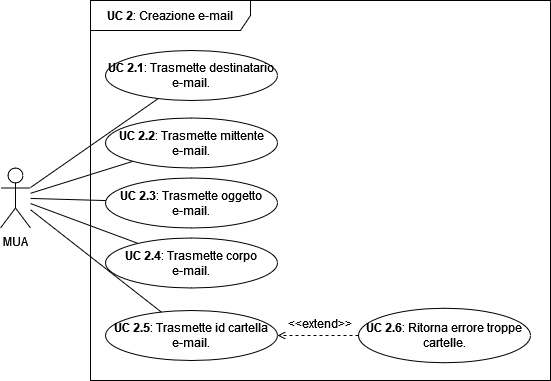
\includegraphics[width=0.85\textwidth]{sections/uc_imgs/UC02.png}
        \centering
        \caption{Diagramma UC 2.}
    \end{figure}
    \begin{itemize}
        \item \textbf{Attore principale}: MUA;
        \item \textbf{Descrizione}: il MUA deve poter inviare una e-mail al destinatario indicato;
        \item \textbf{Precondizioni}: l’account che il MUA gestisce è registrato nel sistema, e ha un connessione aperta con il sistema ed è autenticato;
        \item \textbf{Postcondizioni}: l'e-mail è stata consegnata con successo al destinatario, ed è stata salvata nel sistema;
        \item \textbf{Scenario principale}:
            \begin{enumerate}
                \item il MUA trasmette il destinatario dell'e-mail (\hyperref[sec:UC2.1]{UC 2.1});
                \item il MUA trasmette il mittente dell'e-mail (\hyperref[sec:UC2.2]{UC 2.2});
                \item il MUA trasmette l'oggetto dell'e-mail (\hyperref[sec:UC2.3]{UC 2.3});
                \item il MUA trasmette il corpo dell'e-mail (\hyperref[sec:UC2.4]{UC 2.4});
                \item il sistema salva l'e-mail nel mailbox;
                \item il sistema elabora l'inoltro;
            \end{enumerate}
        \item \textbf{Inclusioni}: nessuna;
        \item \textbf{Generalizzazioni}: nessuna;
        \item \textbf{Estensioni}: 
            \begin{enumerate}[label=\alph*.]
                \item il sistema incontra un errore durante il tentativo d'invio dell'e-mail:
                \begin{enumerate}[label=\arabic*.]
                    \item invia l'e-mail con il codice d'errore al MUA (\hyperref[sec:UC2]{UC 2}).
                \end{enumerate}
            \end{enumerate}
    \end{itemize}

    \begin{figure}[h]
        %\includegraphics[width=0.75\textwidth]{sections/uc_imgs/UC02.X.png}
        \centering
        \caption{Diagramma sotto-casi UC 2.}
    \end{figure}

    \subsubsection{UC 2.1 - Trasmette il destinatario dell'e-mail} \label{sec:UC2.1}
    \begin{itemize}
        \item \textbf{Attore}: MUA;
        \item \textbf{Descrizione}: il MUA invia al sistema il destinatario dell'e-mail;
        \item \textbf{Precondizioni}: il MUA sta usando la funzionalità d'invio di un'e-mail;
        \item \textbf{Postcondizioni}: il sistema conosce l'indirizzo di posta elettronica del destinatario dell'e-mail;
        \item \textbf{Scenario principale}:
            \begin{enumerate}
                \item il MUA trasmette il destinatario, deve soddisfare il seguente requisito:
                    \begin{itemize}
                        \item l'indirizzo e-mail deve essere sintatticamente valido;
                    \end{itemize}
            \end{enumerate}
        \item \textbf{Inclusioni}: nessuna;
        \item \textbf{Generalizzazioni}: nessuna;
        \item \textbf{Estensioni}:
            \begin{enumerate}[label=\alph*.]
                \item l'indirizzo e-mail non è sintatticamente valido:
                \begin{enumerate}[label=\arabic*.]
                    \item il sistema invia un messaggio di errore al MUA (\hyperref[sec:UC2.6]{UC 2.6}).
                \end{enumerate}
            \end{enumerate}
    \end{itemize}

    \subsubsection{UC 2.2 - Trasmette il mittente dell'e-mail} \label{sec:UC2.2}
    \begin{itemize}
        \item \textbf{Attore}: MUA;
        \item \textbf{Descrizione}: il MUA invia al sistema il mittente dell'e-mail;
        \item \textbf{Precondizioni}: il MUA sta usando la funzionalità d'invio di un'e-mail;
        \item \textbf{Postcondizioni}: il sistema conosce l'indirizzo di posta elettronica del mittente dell'e-mail;
        \item \textbf{Scenario principale}:
            \begin{enumerate}
                \item il MUA trasmette il mittente, deve soddisfare il seguente requisito:
                    \begin{itemize}
                        \item l'indirizzo e-mail deve essere sintatticamente valido;
                    \end{itemize}
            \end{enumerate}
        \item \textbf{Inclusioni}: nessuna;
        \item \textbf{Generalizzazioni}: nessuna;
        \item \textbf{Estensioni}:
            \begin{enumerate}[label=\alph*.]
                \item l'indirizzo e-mail non è sintatticamente valido:
                \begin{enumerate}[label=\arabic*.]
                    \item il sistema invia un messaggio di errore al MUA (\hyperref[sec:UC2.7]{UC 2.7}).
                \end{enumerate}
            \end{enumerate}
    \end{itemize}

    \subsubsection{UC 2.3 - Trasmette l'oggetto dell'e-mail} \label{sec:UC2.3}
    \begin{itemize}
        \item \textbf{Attore}: MUA;
        \item \textbf{Descrizione}: il MUA invia al sistema l'oggetto dell'e-mail;
        \item \textbf{Precondizioni}: il MUA sta usando la funzionalità d'invio di un'e-mail;
        \item \textbf{Postcondizioni}: il sistema conosce l'oggetto dell'e-mail;
        \item \textbf{Scenario principale}:
            \begin{enumerate}
                \item il MUA trasmette l'oggetto dell'e-mail;
            \end{enumerate}
        \item \textbf{Inclusioni}: nessuna;
        \item \textbf{Generalizzazioni}: nessuna;
        \item \textbf{Estensioni}: nessuna.
    \end{itemize}

    \subsubsection{UC 2.4 - Trasmette il corpo dell'e-mail} \label{sec:UC2.4}
    \begin{itemize}
        \item \textbf{Attore}: MUA;
        \item \textbf{Descrizione}: il MUA invia al sistema il corpo dell'e-mail;
        \item \textbf{Precondizioni}: il MUA sta usando la funzionalità d'invio di un'e-mail;
        \item \textbf{Postcondizioni}: il sistema conosce il corpo dell'e-mail;
        \item \textbf{Scenario principale}:
            \begin{enumerate}
                \item il MUA trasmette il corpo dell'e-mail;
            \end{enumerate}
        \item \textbf{Inclusioni}: nessuna;
        \item \textbf{Generalizzazioni}: nessuna;
        \item \textbf{Estensioni}: nessuna.
    \end{itemize}



    \subsubsection{UC 2.5 - Ritorna l'errore destinatario non valido} \label{sec:UC2.5}
    \begin{itemize}
        \item \textbf{Attore}: MUA;
        \item \textbf{Descrizione}: il MUA riceve l'errore che il destinatario non è valido;
        \item \textbf{Precondizioni}: il MUA ha inviato il destinatario;
        \item \textbf{Postcondizioni}: il MUA viene notificato che il destinatario non è valido;
        \item \textbf{Scenario principale}:
            \begin{enumerate}
                \item il sistema controlla la sintassi del destinatario e trova un errore;
                \item il sistema notifica il MUA che il destinatario non è valido;
            \end{enumerate}
        \item \textbf{Inclusioni}: nessuna;
        \item \textbf{Generalizzazioni}: nessuna;
        \item \textbf{Estensioni}: nessuna.
    \end{itemize}

    \subsubsection{UC 2.6 - Ritorna l'errore mittente non valido} \label{sec:UC2.6}
    \begin{itemize}
        \item \textbf{Attore}: MUA;
        \item \textbf{Descrizione}: il MUA riceve l'errore che il mittente non è valido;
        \item \textbf{Precondizioni}: il MUA ha inviato il mittente;
        \item \textbf{Postcondizioni}: il MUA viene notificato che il mittente non è valido;
        \item \textbf{Scenario principale}:
            \begin{enumerate}
                \item il sistema controlla la sintassi del mittente e trova un errore;
                \item il sistema notifica il MUA che il mittente non è valido;
            \end{enumerate}
        \item \textbf{Inclusioni}: nessuna;
        \item \textbf{Generalizzazioni}: nessuna;
        \item \textbf{Estensioni}: nessuna.
    \end{itemize}
